\scanpage{9}
\mspage{3}

B) Courbes \inserted{ell.} \unsure{anharmoniques} de type hexagonal.

La catégorie de ces courbes équivaut à celle des hexagones orientés, i.e. des torseurs $S$ sous
\[
\begin{aligned}
\mathbb Z/6\mathbb Z&\simeq\mu_6(\mathbb C)\simeq
\text{groupe des unités \inserted{\unsure{alg.}} de }Q(\underbrace{\sqrt[3]{1}}_{\zeta})\\
&\simeq\text{groupe des unités de}\\
&\qquad \deleted{\mathbb Z[\zeta]\unsure{=}\mathbb Z[T]/}\\
&\qquad \mathbb Z[\zeta]=\mathbb Z[T]/(1+T+T^2)\\
&\qquad (\zeta\unsure{=|:}\exp 2i\pi/3)
\end{aligned}
\]

\figure{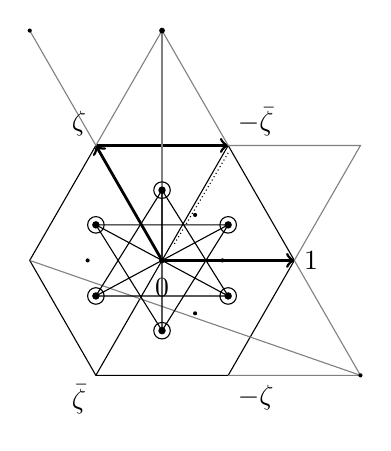
\begin{tikzpicture}[scale=1.05]
\coordinate (O) at (0,0);
\coordinate (A) at (1.6,0);
\coordinate (B) at (.8,1.39);
\coordinate (C) at (-.8,1.39);
\coordinate (D) at (-1.6,0);
\coordinate (E) at (-.8,-1.39);
\coordinate (F) at (.8,-1.39);
\draw (A)--(B)--(C)--(D)--(E)--(F)--cycle;
\draw[line width=1pt,->] (O)--(A);
\draw[line width=1pt,->] (O)--(C);
\draw[line width=1pt,->] (C)--(B);
\draw (E)--(O)--(B);
\draw[densely dotted] (.15,.2)--(.8,1.3);
\draw[thin,gray] (-1.6,2.78)--(C)--(0,2.78)--(B);
\draw[thin,gray] (0,2.78)--(0,0);
\draw[thin,gray] (A)--(2.4,-1.39)--(F);
\draw[thin,gray] (D)--(2.4,-1.39);
\draw[thin,gray] (A)--(2.4,1.39)--(B);
\fill (0,2.78) circle (.035);
\fill (-1.6,2.78) circle (.025);
\fill (2.4,-1.39) circle (.025);
\foreach \p in {(0,.85),(.8,.43),(.8,-.43),(0,-.85),(-.8,-.43),(-.8,.43)}{
 \draw \p circle (.10);
 \fill \p circle (.045);
}
\draw[thin] (0,.85)--(.8,-.43)--(-.8,-.43)--cycle;
\draw[thin] (0,-.85)--(.8,.43)--(-.8,.43)--cycle;
\draw[thin] (0,.85)--(0,-.85) (-.8,.43)--(.8,-.43) (-.8,-.43)--(.8,.43);
\foreach \p in {(-.9,0),(.73,0),(.4,.55),(.4,-.64)}\fill \p circle (.025);
\fill (O) circle (.035);
\node[below] at (0,-.10) {$\unsure{0}$};
\node[right] at (A) {$1$};
\node[above left] at (C) {$\zeta$};
\node[above right] at (B) {$-\bar\zeta$};
\node[below left] at (E) {$\bar\zeta$};
\node[below right] at (F) {$-\zeta$};
\end{tikzpicture}}

\deleted{\unsure{On pourra}} \inserted{On pose}
\[
\mathbb E\ell_1\deleted{(\unsure{S})}\simeq\mathbb C/\mathbb Z[\zeta]
\]
\[
\mathbb E\ell_1(S)\simeq\mathbb E\ell_1\mathbin{\wedge}_{\mathbb Z/6\mathbb Z}S
\]

\uline{Construction} On réalise l'hexagone orient. $S$ \unsure{euclidiennement} (canonique), \unsure{dans} \unsure{vectoriel} euclidien $V_S$, \deleted{\unsure{centre}} \inserted{origine} étant le barycentre de $S$. On désigne par $\unsure{V_S|\Gamma_S}$ le \deleted{\unsure{lattice}} \inserted{réseau} engendré par $S$, et
\[
X_S=\mathbb E\ell_1(S)\simeq V_S/\Gamma_S
\]
La structure euclidienne \uline{orientée} de $V_S$ définit la structure complexe de $X_S$.

\margin{8}
